\documentclass[12pt,a4paper]{article}
\usepackage[utf8]{vietnam}
\usepackage{amsmath}
\usepackage{amsfonts}
\usepackage{xcolor}
\usepackage{titlesec}
\usepackage{mdframed}
\usepackage{amssymb}
\usepackage{graphicx}
\usepackage{cases} 
\usepackage{pgfplots}
\pgfplotsset{compat=1.5}
\usepackage{mathrsfs}
\usetikzlibrary{arrows}
\usepackage{fancyhdr}
\usepackage{float}
\usepackage{enumerate}
\usepackage{enumitem}
\usepackage{diagbox}
\pagestyle{fancy}
\pagestyle{empty}
\usepackage[left=2cm,right=2cm,top=2cm,bottom=2cm]{geometry}
\author{Nguyễn Văn Lộc}
\newmdenv[linecolor=black,skipabove=\topsep,skipbelow=\topsep,
leftmargin=-5pt,rightmargin=-5pt,
innerleftmargin=5pt,innerrightmargin=5pt]{mybox}
\usepackage{tikz,tkz-euclide}
\usetikzlibrary{calc,intersections,patterns}
%\usetkzobj{all}
\begin{document}
    \fancyhf{}
    \lhead{}
    \chead{}
    \rhead{}
    \cfoot{}
    \rfoot{\thepage}
    \lfoot{}
    \pagestyle{fancy}
    \renewcommand{\headrulewidth}{0pt}
    \renewcommand{\footrulewidth}{0pt}
    \begin{mybox}
    \textbf{Họ và tên:} Nguyễn Văn Lộc\\
    \textbf{MSSV:} 20120131\\
    \textbf{Lớp:} 20CTT1
    \end{mybox}
    \begin{center}
    \fontsize{16}{14}\selectfont
    \textbf{Bài tập môn Xác suất thống kê}\\
    \textbf{Chương 2: Biến ngẫu nhiên - Vector ngẫu nhiên}\\
    \textbf{Ngày 07/10/2021}
    \end{center}
    \begin{mybox}
        \textbf{Bài 1.} Dòng điện trong một mạch nhất định được đo bằng một ampere kế là biến ngẫu nhiên liên tục $X$ với hàm mật độ như sau:
        $$f \left( x \right) = 
        \begin{cases}
            0.075x + 0.2, &\text{khi } 3 \leqslant x \leqslant 5\\
            0, &\text{nơi khác}
        \end{cases}
        .$$
    a. Tính $\mathbb{P} \left( {X \leqslant 4} \right)$ và so sánh với xác suất $\mathbb{P} \left( {X > 4} \right).$\\
    b. Tính xác suất $\mathbb{P} \left( {3.5 \leqslant X \leqslant 4.5} \right)$ và so sánh với xác suất $\mathbb{P} \left( {X > 4.5} \right).$
    \end{mybox}
    a. $\mathbb{P} \left( {X \leqslant 4} \right) = \int\limits_{ - \infty }^4 {f\left( x \right)dx}  = \int\limits_{ - \infty }^3 {0dx}  + \int\limits_3^4 {\left( {0.075x + 0.2} \right) \mathrm{d}x}  = 0.4625$\\
    $\Rightarrow \mathbb{P} \left( {X > 4} \right) = 1 - 0.4625 = 0.5375$\\
    $\Rightarrow \mathbb{P} \left( {X \leqslant 4} \right) < \mathbb{P} \left( {X > 4} \right).$\\
    b. $\mathbb{P} \left( {3.5 \leqslant X \leqslant 4.5} \right) = \int\limits_{3.5}^{4.5} {\left( {0.075x + 0.2} \right) \mathrm{d}x}  = 0.5$\\
    $\mathbb{P} \left( {X \leqslant 4.5} \right) = \int\limits_{ - \infty }^4.5 {f\left( x \right)dx}  = \int\limits_{ - \infty }^3 {0dx}  + \int\limits_3^4.5 {\left( {0.075x + 0.2} \right)}  = 0.721875$\\
    $\Rightarrow \mathbb{P} \left( {3.5 \leqslant X \leqslant 4.5} \right) >\mathbb{P} \left( {X > 4.5} \right).$ 

    \begin{mybox}
        \textbf{Bài 2.} Cho $X$ là biến ngẫu nhiên có phân phối xác suất
            \begin{table}[H]
                \begin{center}
                    \begin{tabular}{|c|c|c|c|c|c|c|c|}
                        \hline 
                        $X$ & 1 & 2 & 3 & 4 & 5 & 6 & 7 \\ 
                        \hline 
                        $p$ & $a$ & $2a$ & $2a$ & $3a$ & $a^2$ & $2 a^2$  & $7a^2 + a$ \\ 
                        \hline 
                        \end{tabular}
                \end{center}
            \end{table}
            a. Xác định $a.$\\
            b. Tính $\mathbb{P} \left( {X \geqslant 5} \right)$ và $\mathbb{P} \left( {X > 3} \right).$\\
            c. Tìm $k$ nhỏ nhất sao cho $\mathbb{P} \left( {X \leqslant k } \right) \geqslant \frac{1}{2}.$
    \end{mybox}
    a. $$a + 2a + 2a + 3a + {a^2} + 2{a^2} + 7{a^2} + a = 1$$
    $$\Leftrightarrow a = 0.1,\left( \text{vì } {a \geqslant 0} \right).$$
    b. Hàm phân phối xác suất của $X$ như sau:
    $$F \left( x \right) = 
    \begin{cases}
        0, &\text{nếu } x < 1\\
        0.1, &\text{nếu } 1 \leqslant x < 2\\
        0.3, &\text{nếu } 2 \leqslant x < 3\\
        0.5, &\text{nếu } 3 \leqslant x < 4\\
        0.8, &\text{nếu } 4 \leqslant x < 5\\
        0.81, &\text{nếu } 5 \leqslant x < 6\\
        0.83, &\text{nếu } 6 \leqslant x < 7\\
        1, &\text{nếu } x \geqslant 7
    \end{cases}.$$ 
    $F \left( 3 \right) = 0.5 \Rightarrow \mathbb{P} \left( {X \leqslant 3} \right) = 0.5$\\
    $F \left( 5 \right) = 0.81 \Rightarrow \mathbb{P} \left( {X \leqslant 5} \right) = 0.81 \Rightarrow \mathbb{P} \left( {X > 5} \right) = 0.19$
    c. Dựa vào hàm phân phối xác suất của $X,$ ta được $k = 3.$

\begin{mybox}
   \textbf{Bài 3.} Cho hai biến ngẫu nhiên độc lập $X$ và $Y$ có bảng phân phối xác suất như sau.
    \begin{table}[H]
        \begin{center}
            \begin{tabular}{|c|c|c|c|c|}
                \hline 
                $X$ & -1 & 0 & 1 & 2 \\ 
                \hline 
                $p$ & 0.3 & 0.2 & 0.3 & 0.2 \\ 
                \hline 
                \end{tabular}  
        \end{center}
    \end{table}

    \begin{table}[H]
        \begin{center}
            \begin{tabular}{|c|c|c|c|}
                \hline 
                $Y$ & -1 & 0 & 1 \\ 
                \hline 
                $p$ & 0.3 & 0.4 & 0.3 \\ 
                \hline 
                \end{tabular} 
        \end{center}
    \end{table}
    Lập bảng phân phối xác suất của $X + Y$ và $XY.$
\end{mybox}
Bảng phân phối xác suất của $X + Y.$
\begin{table}[H]
    \begin{center}
        \begin{tabular}{|c|c|c|c|c|c|c|}
            \hline 
            $X + Y$ & -2 & -1 & 0 & 1 & 2 & 3 \\ 
            \hline 
            $p$ & 0.09 & 0.18 & 0.26 & 0.24 & 0.17 & 0.06 \\ 
            \hline 
            \end{tabular} 
    \end{center}
\end{table}
Bảng phân phối xác suất của $XY.$
\begin{table}[H]
    \begin{center}
        \begin{tabular}{|c|c|c|c|c|c|}
            \hline 
            $XY$ & -2 & -1 & 0 & 1 & 2 \\ 
            \hline 
            $p$ & 0.06 & 0.18 & 0.52 & 0.18 & 0.06 \\ 
            \hline 
            \end{tabular} 
    \end{center}
\end{table}

\begin{mybox}
    \textbf{Bài 4.} Linda là một nhân viên bán hàng tại một đại lý ô tô lớn. Với mức hoa hồng $25\%$ lợi nhuận tính trên 
    mỗi chiếc xe cô bán, Linda dự kiến sẽ kiếm được $350\$ $ cho mỗi chiếc xe hơi bán được và $400\$ $ cho mỗi 
    chiếc xe tải hoặc SUV bán được. Linda thúc đẩy bản thân bằng cách sử dụng ước lượng xác suất cho 
    doanh thu của mình. Vào một ngày Thứ Bảy của tháng Tư, cô ước tính doanh số bán xe hơi và xe tải hoặc SUV của mình như sau:
    Đặt $X$ là số xe hơi Linda bán và $Y$ là số xe tải hoặc SUV.
    \begin{table}[H]
        \begin{center}
            \begin{tabular}{|c|c|c|c|c|}
                \hline 
                $X$ & 0 & 1 & 2 & 3 \\ 
                \hline 
                $p$ & 0.3 & 0.4 & 0.2 & 0.1 \\ 
                \hline 
                \end{tabular} 
        \end{center}
    \end{table}
    \begin{table}[H]
        \begin{center}
            \begin{tabular}{|c|c|c|c|}
                \hline 
                $Y$ & 0 & 1 & 2 \\ 
                \hline 
                $p$ & 0.4 & 0.5 & 0.1 \\ 
                \hline 
                \end{tabular} 
        \end{center}
    \end{table}
    a. Hãy tính trung bình lượng xe mỗi loại cô bán, từ đó suy ra doanh thu trung bình cô thu được.\\
    b. Tính phương sai và độ lệch chuẩn cho biến $X.$
\end{mybox}
a. $\mathbb{E} \left( X \right) = 0 \cdot 0.3 + 1 \cdot 0.4 + 2 \cdot 0.2 + 3 \cdot 0.1 = 1.1$\\
$\Rightarrow$ Trung bình Linda bán được $1.1$ chiếc xe hơi, kiếm được $385 \$.$\\
$\mathbb{E} \left( Y \right) = 0 \cdot 0.4 + 1 \cdot 0.5 + 2 \cdot 0.1 = 0.7$\\
$\Rightarrow$ Trung bình Linda bán được $0.7$ chiếc xe tải hoặc SUV, kiếm được $280 \$.$\\
b. Bảng phân phối xác suất của $X^2$ như sau:
\begin{table}[H]
    \begin{center}
        \begin{tabular}{|c|c|c|c|c|}
            \hline 
            $X^2$ & 0 & 1 & 4 & 9 \\ 
            \hline 
            $p$ & 0.3 & 0.4 & 0.2 & 0.1 \\ 
            \hline 
            \end{tabular} 
    \end{center}
\end{table}
$\mathbb{E} \left( {X^2} \right) = 0 \cdot 0.3 + 1 \cdot 0.4 + 4 \cdot 0.2 + 9 \cdot 0.1 = 2.1$\\
$\mathbb{V}ar \left( X \right) = \mathbb{E} \left( {X^2} \right) - \left( {\mathbb{E} \left( {X^2} \right)} \right)^2 = 0.89$\\
$\sigma \left( X \right) = \frac{\sqrt{89}}{10}.$


\begin{mybox}
    \textbf{Bài 5.} 
    Một  nhà  sản  xuất  ổ  đĩa  bán  ra  các  thiết  bị  lưu  trữ  với  dung  lượng  1  terabyte,  500 
    gigabyte và 100 gigabyte với tỷ lệ tương ứng là $50\%$, $30\%$ và $20\%$. Doanh thu ước tính trong năm tương 
    ứng với từng thiết bị bán ra là 50 triệu $\$$, 25 triệu $\$$ và 10 triệu $\$$. Xác định hàm xác suất, hàm 
    phân phối cho doanh thu của thiết bị lưu trữ trong năm đó. Tính doanh thu trung bình của thiết bị lưu trữ trong năm đó.  
\end{mybox}
Gọi $X$ là doanh thu của nhà sản xuất, đơn vị triệu $S$. Bảng phân phối xác suất của $X$ như sau:
\begin{table}[H]
    \begin{center}
        \begin{tabular}{|c|c|c|c|c|}
            \hline 
            $X^2$ & 10 & 25 & 30 \\ 
            \hline 
            $p$ & 0.2 & 0.3 & 0.5  \\ 
            \hline 
            \end{tabular} 
    \end{center}
\end{table}
Hàm phân phối xác suất của $X$ là:
$$F \left( x \right) = 
\begin{cases}
    0,&\text{nếu } x < 10\\
    0.2,&\text{nếu } 10 \leqslant x < 25\\
    0.5,&\text{nếu } 25 \leqslant x < 50\\
    1,&\text{nếu } x \geqslant 50
\end{cases}
.$$
Doanh thu trung bình của nhà sản xuất trong năm đó là:
$$\mathbb{E} \left( X \right) = 10 \cdot 0.2 + 25 \cdot 0.3 + 50 \cdot 0.5 = 234.5 \left( {\text{triệu } \$} \right).$$

\begin{mybox}
\textbf{Bài 6.} Đặt ngẫu nhiên mỗi một trái banh trong ba trái banh đang có vào một trong ba cái
chén. Tìm phân phối xác suất cho $Y$ với $Y$ là số cái chén trống.
\end{mybox}
Gọi $x_1, x_2, x_3$ với $x_i \geqslant 0$ là số trái banh trong chén thứ $i.$
Ta có $x_1 + x_2 + x_3 = 3.$ Phương trình này có số lượng nghiệm nguyên không âm là: $K^3_3 = 10.$\\
\textbf{\underline{Trường hợp 1:}} Không có cái chén nào rỗng.\\
Trong trường hợp này, mỗi cái chén chứa đúng một trái banh. Số cách chọn là $1.$ Xác suất cho trường hợp này là $p_1= \frac{1}{10} = 0.1$\\
\textbf{\underline{Trường hợp 2:}} Có một cái chén rỗng.\\
Trong hai cái chén còn lại, có một cái chén chứa hai trái banh. Số cách chọn cho trường hợp này là $C^1_3 \cdot C^1_2 = 6.$ Xác suất cho trường hợp này là $p_2 = \frac{6}{10} = 0.6$\\
\textbf{\underline{Trường hợp 3:}} Có hai cái chén rỗng.\\
Số cách chọn cho trường hợp này là $C^2_3 = 3.$ Xác suất cho trường hợp này là $p_3 = \frac{3}{10} = 0.3$\\
Bảng phân phối xác suất cho $Y$ nhưu sau
\begin{table}[H]
    \begin{center}
        \begin{tabular}{|c|c|c|c|c|}
            \hline 
            $Y$ & 0 & 1 & 2 \\ 
            \hline 
            $p$ & 0.1 & 0.6 & 0.3  \\ 
            \hline 
            \end{tabular} 
    \end{center}
\end{table}

\begin{mybox}
    \textbf{Bài 7.} .  Một giáo sư đại học không bao giờ kết thúc bài giảng của mình trước khi hết giờ và luôn  hoàn  
    thành  bài  giảng  của  mình  trong  vòng  $2$  phút  sau  giờ  học.  Cho  $X$  là  thời gian trôi qua 
    giữa thời điểm hết tiết học và kết thúc bài giảng của giáo sư. Giả sử hàm mật độ của $X$  là:
    $$f \left( x \right) = 
    \begin{cases}
        kx^2,&\text{khi } 0 \leqslant x \leqslant 2\\
        0,&\text{nơi khác}
    \end{cases}
    .$$
    a. Tìm $k.$\\
    b. Hãy tính xác suất bài giảng kết thúc trong vòng $1$ phút sau khi giờ học kết thúc.\\
    c. Hãy tính xác suất bài giảng tiếp tục diễn ra sau khi giờ học kết thúc từ $60 \mathrm{s}$ đến $90 \mathrm{s}.$\\
    d. Xác suất mà bài giảng tiếp tục trong ít nhất $90 \mathrm{s}$ ngoài giờ kết thúc là bao nhiêu?
\end{mybox}
a. $f \left( x \right)$ là hàm mật độ xác suất
$$ \Leftrightarrow \int\limits_{ - \infty }^\infty  {f\left( x \right)\mathrm{d}x} = 1 $$
$$ \Leftrightarrow \int\limits_{ - \infty }^0 {0\mathrm{d}x}  + \int\limits_0^2 {k{x^2}\mathrm{d}x}  + \int\limits_2^\infty  {0\mathrm{d}x}  = 1$$
$$ \Leftrightarrow \frac{{8k}}{3} = 1 \Leftrightarrow k = \frac{3}{8}.$$
b. $$\mathbb{P} \left( { X \leqslant 1 }\right) = \int\limits_{- \infty}^1 {f\left( x \right)\mathrm{d}x}$$
$$ = \int\limits_{0}^1 {\frac{3}{8} x^2 \mathrm{d}x} = \frac{1}{8}.$$
c. $$\mathbb{P} \left( {1 \leqslant X \leqslant 1.5 }\right) = \int\limits_{1}^{1.5} {\frac{3}{8} x^2 \mathrm{d}x} = \frac{19}{64}.$$
d. $$\mathbb{P} \left( { X \leqslant 1.5 }\right) = \int\limits_{- \infty}^{1.5} {f\left( x \right)\mathrm{d}x}$$
$$ = \int\limits_{0}^{1.5} {\frac{3}{8} x^2 \mathrm{d}x} = \frac{27}{64}$$
$$\Rightarrow \mathbb{P} \left( { X \geqslant 1.5 }\right) = \frac{37}{64}.$$

\begin{mybox}
    \textbf{Bài 8.} Cho biến ngẫu nhiên $X$ có hàm mật độ xác suất như sau:
    $$f \left( x \right) = 
    \begin{cases}
        6x \left( {1 - x} \right), &\text{ nếu } x \in \left[ {0, 1} \right]\\
        0, &\text{nơi khác}
    \end{cases}
    .$$
    a. Tìm hàm mật độ xác suất của biến ngẫu nhiên $Y = 2X - 3.$\\
    b. Tính $\mathbb{E} \left( X \right), \mathbb{E} \left( Y \right), \mathbb{V} \left( X \right), \mathbb{V} \left( Y \right).$
\end{mybox}
a. Gọi $G$ là hàm phân phối xác suất của biến ngẫu nhiên $Y.$\\
$$G \left( y \right) = \mathbb{P} \left( {Y \leqslant y} \right) = \mathbb{P} \left( {2X - 3 \leqslant y} \right)$$
$$ =  \mathbb{P} \left( {X \leqslant \frac{y + 3}{2}} \right)$$
\textbf{\underline{Trường hợp 1: }} $y < -3.$ $G \left( y \right) = 0.$\\
\textbf{\underline{Trường hợp 2: }} $-3 \leqslant y \leqslant -1.$ 
$$G \left( y \right) = \int\limits_{- \infty}^{\frac{y + 3}{2}}{f \left(x \right) \mathrm{d}x} = \int\limits_{0}^{\frac{y + 3}{2}}{6x \left( {1 - x} \right)\mathrm{d}x}$$
$$ = \left. {\left( {3{x^2} - 2{x^3}} \right)} \right|_0^{\frac{{y + 3}}{2}} =  - \frac{{{y^3} + 6{y^2} + 9y}}{4}$$
\textbf{\underline{Trường hợp 3: }} $y >= -1.$ $G \left( y \right) = 1.$\\
Vậy hàm mật độ xác suất của biến ngẫu nhiên $Y$ là:
$$g \left( y \right) = 
    \begin{cases}
        - \frac{3y^2 + 12y + 9}{4}, &\text{ nếu } y \in \left[ {-3, -1} \right]\\
        0, &\text{nơi khác}
    \end{cases}
    .$$

b. $$\mathbb{E} \left( X \right) = \int\limits_0^1 {x \cdot 6x\left( {1 - x} \right)\mathrm{d}x}  = \frac{1}{2}$$
$$\mathbb{E} \left( {{X^2}} \right) = \int\limits_0^1 {{x^2} \cdot 6x\left( {1 - x} \right)\mathrm{d}x}  = \frac{3}{{10}}$$
$$\mathbb{E} \left( Y \right) = \int\limits_{ - 3}^{ - 1} {y \cdot \left( { - \frac{{3{y^2} + 12y + 9}}{4}} \right)} \mathrm{d}y =  - 2$$
$$\mathbb{E} \left( {{Y^2}} \right) = \int\limits_{ - 3}^{ - 1} {{y^2} \cdot \left( { - \frac{{3{y^2} + 12y + 9}}{4}} \right)} \mathrm{d}y = \frac{{21}}{5}$$
$$\mathbb{V} \left( X \right) = \mathbb{E} \left( {{X^2}} \right) - \left( {\mathbb{E} \left( X \right)}\right)^2 = \frac{1}{20}.$$
$$\mathbb{V} \left( Y \right) = \mathbb{E} \left( {{Y^2}} \right) - \left( {\mathbb{E} \left( Y \right)}\right)^2 = \frac{1}{5}.$$

\begin{mybox}
    \textbf{Bài 9.} Cho biến ngẫu nhiên $X$ có hàm phân phối:
    $$F \left( x \right) = 
    \begin{cases}
        0, &\text{nếu } x < 0\\
        1, &\text{nếu } x > \frac{\pi}{4}\\
        \sin \left( {2x} \right), &\text{nếu } 0 \leqslant x \leqslant \frac{\pi}{4}
    \end{cases}
    .$$
    a. Tìm hàm mật độ xác suất của $X.$\\
    b. Tính $\mathbb{P} \left( {-\frac{\pi}{6} \leqslant X \leqslant \frac{\pi}{4}}\right)$.
\end{mybox}
a. Hàm mật độ xác suất của $X$ là:
$$f \left( x \right) = 
    \begin{cases}
        2 \cos \left( {2x} \right), &\text{nếu } 0 \leqslant x \leqslant \frac{\pi}{4}\\
        0, &\text{nơi khác }
        
    \end{cases}
    .$$
b. $$\mathbb{P} \left( {-\frac{\pi}{6} \leqslant X \leqslant \frac{\pi}{4}}\right) = \int\limits_{-\frac{\pi}{6}}^{\frac{\pi}{4}}{f \left( x \right) \mathrm{d}x}$$
$$ = \int\limits_{0}^{\frac{\pi}{4}}{2 \cos \left( {2x} \right)\mathrm{d}x}  = 1.$$

\begin{mybox}
    \textbf{Bài 10.} Cho bảng phân phối xác suất đồng thời của $X$ và $Y$
    \begin{table}[H]
        \begin{center}
            \begin{tabular}{|c|c|c|c|}
                \hline 
                \diagbox{$X$}{$Y$} & 1.5 & 2 & 3.5 \\ 
                \hline 
                1 & $3\lambda$ & $\lambda$ & 0 \\ 
                \hline 
                2 & $2\lambda$ & $4\lambda$ & $2\lambda$ \\ 
                \hline 
                4 & $\lambda$ & $2\lambda$ & $5\lambda$ \\ 
                \hline 
                \end{tabular} 
        \end{center}
    \end{table}
    a. Xác định hằng số $\lambda.$\\
    b. Tìm các phân phối lề của biến ngẫu nhiên $X$ và biến ngẫu nhiên $Y.$\\
    c. Tìm hàm mật độ có điều kiện của $Y$ khi biết $X = x$ và hàm mật độ có điều kiện của $X$ khi $Y = y.$
\end{mybox}
a. Tổng xác suất trong bảng bằng $1$ nên:
$$ 3\lambda + \lambda + 2\lambda + 4\lambda + 2\lambda + \lambda + 2\lambda + 5\lambda = 1$$
$$\Leftrightarrow \lambda = 0.05$$
b. Bảng phân phối lề của biến ngẫu nhiên $X$:
\begin{table}[H]
    \begin{center}
        \begin{tabular}{|c|c|c|c|c|}
            \hline 
            $X$ & 1 & 2 & 4 \\ 
            \hline 
            $f_X \left( X \right)$ & 0.2 & 0.4 & 0.4  \\ 
            \hline 
            \end{tabular} 
    \end{center}
\end{table}
Bảng phân phối lề của biến ngẫu nhiên $Y$:
\begin{table}[H]
    \begin{center}
        \begin{tabular}{|c|c|c|c|c|}
            \hline 
            $Y$ & 1 & 2 & 4 \\ 
            \hline 
            $f_Y \left( y \right)$ & 0.3 & 0.35 & 0.35  \\ 
            \hline 
            \end{tabular} 
    \end{center}
\end{table}
c. ${f_{\left. X \right|Y}}\left( {\left. x \right|y} \right)$
\begin{table}[H]
    \begin{center}
        \begin{tabular}{|c|c|c|c|}
            \hline 
            \diagbox{$X$}{$Y$} & 1.5 & 2 & 3.5 \\ 
            \hline 
            1 & $0.75$ & $0.25$ & $0$ \\ 
            \hline 
            2 & $0.25$ & $0.5$ & $0.25$ \\ 
            \hline 
            4 & $0.125$ & $0.25$ & $0.625$ \\ 
            \hline 
            \end{tabular} 
    \end{center}
\end{table}

${f_{\left. Y \right|X}}\left( {\left. y \right|x} \right)$
\begin{table}[H]
    \begin{center}
        \begin{tabular}{|c|c|c|c|}
            \hline 
            \diagbox{$X$}{$Y$} & 1.5 & 2 & 3.5 \\ 
            \hline 
            1 & $\frac{1}{2}$ & $\frac{1}{7}$ & $0$ \\ 
            \hline 
            2 & $\frac{1}{3}$ & $\frac{4}{7}$ & $\frac{2}{7}$ \\ 
            \hline 
            4 & $\frac{1}{6}$ & $\frac{2}{7}$ & $\frac{5}{7}$ \\ 
            \hline 
            \end{tabular} 
    \end{center}
\end{table}

\begin{center}
    \fontsize{16}{14}\selectfont
    \textbf{Bài tập làm thêm}
\end{center}
\begin{mybox}
    \textbf{Bài tập 2.9} (bài này giống bài 4 ở trên ạ)
\end{mybox}

\begin{mybox}
    \textbf{Bài tập 2.15} (bài này giống bài 5 ở trên ạ) 
\end{mybox}

\begin{mybox}
    \textbf{Bài tập 2.16} Một kết cấu gồm $3$ thành phần cơ khí hoạt động độc lập với nhau. Giả sử rằng xác suất mà các thành phần thứ nhất, thứ hai và thứ
    ba đáp ứng được các chi tiết kỹ thuật lần lượt là $0.95, 0.98, 0.99.$ Tìm hàm xác suất, hàm phân phối xác suất cho số lượng các thành phần đáp ứng chi tiết 
    kỹ thuật trong kết cấu.
\end{mybox}
Gọi $X$ là số lượng thành phần đáp ứng các chi tiết kỹ thuật.\\
\textbf{\underline{Trường hợp 1.}} Không có thành phần nào đáp ứng các chi tiết kỹ thuật.\\
Xác suất cho trường hợp này là $p_1 = 0.05 \cdot 0.02 \cdot 0.01 = \frac{1}{100000}.$\\
\textbf{\underline{Trường hợp 2.}} Có đúng một thành phần đáp ứng các chi tiết kỹ thuật.\\
Xác suất cho trường hợp này là $p_2 = 0.95 \cdot 0.02 \cdot 0.01 + 0.05 \cdot 0.98 \cdot 0.01 + 0.05 \cdot 0.02 \cdot 0.99 = \frac{167}{100000}.$\\
\textbf{\underline{Trường hợp 3.}} Có đúng hai thành phần đáp ứng các chi tiết kỹ thuật.
Xác suất cho trường hợp này là $p_3 = 0.95 \cdot 0.98 \cdot 0.01 + 0.95 \cdot 0.02 \cdot 0.99 + 0.05 \cdot 0.98 \cdot 0.99 = \frac{7663}{100000}.$\\
\textbf{\underline{Trường hợp 4.}} Cả ba thành phần đều đáp ứng các chi tiết kỹ thuật.\\
Xác suất cho trường hợp này là $p_4 = 0.95 \cdot 0.98 \cdot 0.99 = \frac{92169}{100000}.$\\
Do đó, ta có bảng phân phối xác suất của biến ngẫu nhiên $X$ như sau:
\begin{table}[H]
    \begin{center}
        \begin{tabular}{|c|c|c|c|c|}
            \hline 
            $X$ & 0 & 1 & 2 & 3 \\ 
            \hline 
            $p$ & $\frac{1}{100000}$ & $\frac{167}{100000}$ & $\frac{7663}{100000}$ & $\frac{92169}{100000}$  \\ 
            \hline 
            \end{tabular} 
    \end{center}
\end{table}
Vậy ta được hàm phân phối xác suất của $X$ như sau:
$$F \left( x \right) = 
\begin{cases}
    0, &\text{nếu } x < 0\\
    \frac{1}{100000}, &\text{nếu } 0 \leqslant x < 1\\
    \frac{21}{12500}, &\text{nếu } 1 \leqslant x < 2\\
    \frac{7831}{100000}, &\text{nếu } 2 \leqslant x < 3\\
    1, &\text{nếu } x \geqslant 3
\end{cases}
.$$

\begin{mybox}
    \textbf{Bài tập 2.17} Miền giá trị của biến ngẫu nhiên $Y$ là $\left\{ {0, 1, 2, 3, y} \right\}$ với $y$ chưa biết và $\mathbb{P} \left( {Y = a}\right) = 0.2$
    với $a = 0, 1, 2, 3 , y.$ Tìm $y$ để giá trị trung bình của biến ngẫu nhiên $Y$ là $6.$
\end{mybox}
$$0.2 \left( {0 + 1 + 2 + 3 + y}\right) = 6$$
$$\Leftrightarrow y = 24.$$

\begin{mybox}
    \textbf{Bài tập 2.18} Trong một hộp có hai đồng xu $10$ cent và một đồng xu $50$ cent. Chọn ngẫu nhiên hai đồng xu từ hộp.
    Gọi $X$ là tổng giá trị hai đồng xu lấy ra.\\
    a. $X$ có thể nhận những giá trị nào?\\
    b. Tìm hàm phân phối xác suất của $X.$
\end{mybox}
a. $X$ có thể nhận các giá trị $20, 60.$\\
b. Xác suất cho trường hợp $X$ nhận giá trị $20$ là: $\frac{1}{C_3^1} = \frac{1}{3}.$\\
Xác suất cho trường hợp $X$ nhận giá trị $60$ là: $\frac{C_2^1 }{C_3^1} = \frac{2}{3}.$\\
Bảng phân phối xác suất của $X$ như sau:
\begin{table}[H]
    \begin{center}
        \begin{tabular}{|c|c|c|c|c|}
            \hline 
            $X$ & 20 & 60  \\ 
            \hline 
            $p$ & $\frac{1}{3}$ & $\frac{2}{3}$   \\ 
            \hline 
            \end{tabular} 
    \end{center}
\end{table}
Hàm phân phối xác suất của $X$ như sau:
$$F \left( x \right) = 
\begin{cases}
    0, &\text{ nếu } x < 20\\
    \frac{1}{3}, &\text{ nếu } 20 \leqslant x < 60\\
    1, &\text{ nếu } x >= 60
\end{cases}
.$$

\begin{mybox}
    \textbf{Bài tập 2.19} Sở Y tế kiểm tra hai tạp chất thường thấy trong nước uống ở những giếng tư nhân trong một tỉnh.
    Kết quả kiểm tra cho thấy có $20\%$ các giếng có cả hai tạp chất, $40\%$ các giếng có tạp chất $A,$ $50\%$ các giếng có tạp chất B.
    Nếu chọn ngẫu nhiên một giếng từ các giếng trong tỉnh, tìm phân phối xác suất cho $Y,$ với $Y$ là số tạp chất được tìm thấy trong giếng.
\end{mybox}
Phần trăm số lượng các giếng chỉ có tạp chất $A$ là: $20\%.$\\
Phần trăm số lượng các giếng chỉ có tạp chất $B$ là: $30\%.$\\
Phần trăm số lượng các giếng có cả hai tạp chất là $20\%.$\\
Phần trăm số lượng các giếng không có tạp chất là: $100\% - 20\% - 30\% - 20\% = 30\%.$\\
Vậy bảng phân phối xác suất của $Y$ là:
\begin{table}[H]
    \begin{center}
        \begin{tabular}{|c|c|c|c|c|}
            \hline 
            $Y$ & 0 & 1 & 2  \\ 
            \hline 
            $p$ & 0.3 & 0.5 & 0.2  \\ 
            \hline 
            \end{tabular} 
    \end{center}
\end{table}

\begin{mybox}
    \textbf{Bài tập 2.20} Trong một kiểm tra đưa ra cho các đứa trẻ, có ba tấm hình về các động vật, yêu cầu các đứa trẻ nối một tấm hình đến
    một từ để nhận biết các động vật đó. Nếu một đứa trẻ gán ba từ một cách ngẫu nhiên đến ba hình ảnh, tìm phân phối xác suất cho $Y$ với 
    $Y$ là số lần nhận diện đúng.
\end{mybox}
\textbf{\underline{Trường hợp 1:}} $Y = 3.$ Xác suất cho trường hợp này là $\frac{1}{6}.$\\
Trường hợp $Y = 2$ không xảy ra vì nếu đứa trẻ đó đã nhận diện đúng hai động vật thì động vật thứ ba cũng đúng.\\
\textbf{\underline{Trường hợp 2:}} $Y = 1.$ Xác suất cho trường hợp này là $\frac{1}{2}.$\\
\textbf{\underline{Trường hợp 3:}} $Y = 0.$ Xác suất cho trường hợp này là $\frac{1}{3}.$\\
Bảng phân phối xác suất của $Y$ như sau:
\begin{table}[H]
    \begin{center}
        \begin{tabular}{|c|c|c|c|c|}
            \hline 
            $Y$ & 0 & 1 & 3  \\ 
            \hline 
            $p$ & $\frac{1}{3}$ & $\frac{1}{2}$ & $\frac{1}{6}$  \\ 
            \hline 
            \end{tabular} 
    \end{center}
\end{table}

\begin{mybox}
    \textbf{Bài tập 2.21} (bài này giống bài 6 ở trên ạ)
\end{mybox}

\begin{mybox}
    \textbf{Bài tập 2.26} (bài này giống bài 1 ở trên ạ)
\end{mybox}

\begin{mybox}
    \textbf{Bài tập 2.27} Lỗi liên quan đến việc thực hiện một phép đo nhất định là một biến ngẫu nhiên $X$ với hàm mật độ xác suất:
    $$f \left( x \right) = 
    \begin{cases}
        0.09375 \left( {4 - x^2}\right), &\text{nếu } -2 \leqslant x \leqslant 2\\
        0, &\text{còn lại}
    \end{cases}
    .$$
    a. Hãy vẽ hàm mật độ xác suất của $X.$\\
    b. Tính $\mathbb{P} \left( {X > 0} \right).$\\
    c. Tính $\mathbb{P} \left( {-1 < X < 1} \right).$\\
    d. Tính $\mathbb{P} \left( {X < -0.5 \text{ hoặc } X > 0.5} \right).$
\end{mybox}
a. \begin{center}
    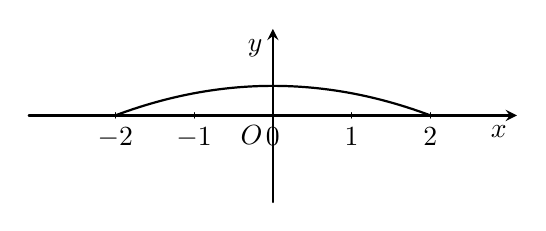
\begin{tikzpicture}[line join=round, line cap=round,>=stealth,thick]
        \tikzset{label style/.style={font=\footnotesize}}
        \draw[->] (-3.1,0)--(3.1,0) node[below left] {$x$};
        \draw[->] (0,-1.1)--(0,1.1) node[below left] {$y$};
        \draw (0,0) node [below left] {$O$};
        \foreach \x in {-2, -1, 0, 1, 2}
            \draw[thin] (\x,1pt)--(\x,-1pt) node [below] {$\x$};
        \begin{scope}
        \clip (-3,-1) rectangle (3,1);
        \draw[samples=200,domain=-2:2,smooth,variable=\x] plot (\x,{-0-0.09375*(\x)^2+0*(\x)+0.375});
        \end{scope}
        \end{tikzpicture}
\end{center}
b. $$\mathbb{P} \left( {X \leqslant 0} \right) = \int\limits_{-2}^{0}{0.09375 \left( {4 - x^2} \right) \mathrm{d}x} = \frac{1}{2}.$$
$$\Rightarrow \mathbb{P} \left( {X > 0} \right) = \frac{1}{2}.$$
c. $$\mathbb{P} \left( {-1 < x < 1} \right) = \int\limits_{-1}^{1}{0.09375 \left( {4 - x^2} \right) \mathrm{d}x} = \frac{11}{16}.$$
d. $$\mathbb{P} \left( {X < -0.5 \text{ hoặc } X > 0.5} \right) = 1 - \int\limits_{-0.5}{0.5}{0.09375 \left( {4 - x^2} \right) \mathrm{d}x} = 1 - \frac{81}{128}.$$

\begin{mybox}
    \textbf{Bài tập 2.28} (bài này giống bài 7 ở trên ạ)
\end{mybox}

\begin{mybox}
    \textbf{Bài tập 2.29} Giả sử nhiệt độ phản ứng $X$ (tính theo $^\circ C$) trong một quá trình phản ứng hóa học nào đó có phân phối đều 
    với $A = -5$ và $B = 5.$\\
    a. Tính $\mathbb{P} \left( { X < 0} \right).$\\
    b. Tính $\mathbb{P} \left( {-2.5 < X < 2.5} \right).$\\
    c. $\mathbb{P} \left( {-2 \leqslant X \leqslant 3} \right).$\\
    d. Với $k$ thỏa $-5 < k < k + 4 < 5,$ hãy tính $\mathbb{P} \left( {k < X < k + 4} \right).$
\end{mybox}
    a. Do $X$ có phân phối đều nên hàm mật độ xác suất của $X$ là:
    $$f \left( x \right) = 
    \begin{cases}
        \frac{1}{10}, &\text{ nếu } -5 \leqslant x \leqslant 5\\
        0, &\text{ còn lại } 
    \end{cases}
    .$$
    $$\mathbb{P} \left( { X < 0} \right) = \int\limits_{-5}^{0}{\frac{1}{10}\mathrm{d}x} = \frac{1}{2}.$$
    b. $$\mathbb{P} \left( {-2.5 < X < 2.5} \right) = \int\limits_{-2.5}^{2.5}{\frac{1}{10}\mathrm{d}x} = \frac{1}{2}.$$
    c. $$\mathbb{P} \left( {-2 \leqslant X \leqslant 3} \right) = \int\limits_{-2}^{3}{\frac{1}{10}\mathrm{d}x} = \frac{1}{2}.$$
    d. $$\mathbb{P} \left( {k < X < k + 4} \right) = \int\limits_{k}^{k + 4}{\frac{1}{10}\mathrm{d}x} = \frac{2}{5}.$$

\begin{mybox}
    \textbf{Bài tập 2.34} Gọi $X$ là tuổi thọ của con người. Một công trình nghiên cứu cho biết hàm mật độ xác suất của $X$ là:
    $$f \left( x \right) = 
    \begin{cases}
        cx^2 \left( {100 - x} \right)^2, &\text{ nếu } 0 \leqslant x \leqslant 100\\
        0, &\text{còn lại.}
    \end{cases}
    .$$
    a. Xác định hằng số $c.$\\
    b. Tính trung bình và phương sai của $X.$\\
    c. Tính xác suất của một người có tuổi thọ $\geqslant 60.$\\
    d. Tính xác suất của một người có tuổi thọ $\geqslant 60,$ biết rằng hiện nay người đó đã $50$ tuổi.
\end{mybox}
a. $$\int\limits_{0}^{100}{cx^2\left( {100 - x} \right)^2 \mathrm{d}x} = 1 \Leftrightarrow c = \frac{3}{10^9}.$$
b. $$\mathbb{E} \left( X \right) = \int\limits_{0}^{100}{x \cdot \frac{3}{10^9} x^2 \left( {100 - x} \right)^2 \mathrm{d}x} = 50.$$
$$\mathbb{E} \left( {X^2} \right) = \int\limits_{0}^{100}{x^2 \cdot \frac{3}{10^9} x^2 \left( {100 - x} \right)^2\mathrm{d}x} = \frac{20000}{7}.$$
$$\mathbb{V} \left( X \right) = \frac{20000}{7} - 50^2 = \frac{2500}{7}.$$
c. $$\mathbb{P} \left( X \leqslant 60 \right) = \int\limits_{0}^{60}{\frac{3}{10^9} x^2 \left( {100 - x} \right)^2\mathrm{d}x} = \frac{2133}{3125}.$$
$$\mathbb{P} \left( X \geqslant 60 \right) = 1 - \frac{2133}{3125} = \frac{992}{3125}.$$
d. $$\mathbb{P} \left( {\left. X \leqslant 60 \right| X \leqslant 50} \right) = \frac{\mathbb{P} \left( X \geqslant 60 \right)}{\mathbb{P} \left( X \geqslant 50 \right)} = \frac{\mathbb{P} \left( X \geqslant 60 \right)}{1 - \mathbb{P} \left( X \leqslant 50 \right)} = \frac{1984}{3125}.$$

\begin{mybox}
    \textbf{Bài tập 2.37} Cho $X$ là một biến ngẫu nhiên có hàm phân phối xác suất như sau:
    $$F \left( x \right) = 
    \begin{cases}
        0, &\text{ nếu } x < 0\\
        \frac{x^2}{4}, &\text{ nếu } 0 \leqslant x \leqslant 2\\
        1, &\text{ nếu } x > 2
    \end{cases}
    .$$
    a. Tính $\mathbb{P} \left( {X \leqslant 1} \right).$\\
    b. Tính $\mathbb{P} \left( {0.5 \leqslant X \leqslant 1} \right).$\\
    c. Tính $\mathbb{P} \left( {X \geqslant 1.5} \right).$\\
    d. Tìm giá trị trung vị của $X.$\\
    e. Tìm hàm mật độ xác suất $f \left( x \right).$\\
    f. Tính $\mathbb{E} \left( X \right).$\\
    g. Tính $\mathbb{V} \left( X \right)$ và $\sigma_X.$\\
    h. Tính trung bình của biến ngẫu nhiên $h \left( X \right) = X^2.$
\end{mybox} 
a. $$\mathbb{P} \left( {X \leqslant 1} \right) = F \left( 1 \right) - F \left( 0 \right) = \frac{1}{4}.$$
b. $$\mathbb{P} \left( {0.5 \leqslant X \leqslant 1} \right) = F \left( 1 \right) - F \left( {0.5} \right) = \frac{3}{16}.$$
c. $$\mathbb{P} \left( {X \geqslant 1.5} \right) = 1 - \mathbb{P} \left( {X < 1.5} \right) = 1 - F \left( {1.5} \right) + F \left( 0 \right) = \frac{7}{16}.$$
d. Giá trị trung vị của $X$ là $x_M$ thỏa: $F \left( {x_M} \right) = \frac{1}{2} \Leftrightarrow x_M = \sqrt{2}.$\\
Vậy $Med \left( X \right) = \sqrt{2}.$\\
e. Hàm mật độ xác suất của $X$ như sau:
$$f \left( x \right) = 
\begin{cases}
    \frac{x}{2}, &\text{ nếu } 0 \leqslant x \leqslant 2\\
    0, &\text{ nơi khác }
\end{cases}
.$$
f. $$\mathbb{E} \left( X \right) = \int\limits_0^2{x \cdot \frac{x}{2} \mathrm{d}x} = \frac{4}{3}.$$
g. $$\mathbb{E} \left( {X^2} \right) = \int\limits_0^2{x^2 \cdot \frac{x}{2} \mathrm{d}x} = 2.$$
$$\mathbb{V} \left( X \right) = \mathbb{E} \left( {X^2} \right) - \left( {\mathbb{E} \left( X \right)} \right)^2 = \frac{2}{9}.$$
$$\Rightarrow \sigma_X = \sqrt{\mathbb{V} \left( X \right)} = \frac{\sqrt{2}}{3}.$$
h. $\mathbb{E} \left( {X^2} \right) = 2.$

\begin{mybox}
    \textbf{Bài tập 2.174} Cho vector ngẫu nhiên có hàm mật độ xác suất đồng thời:
    $$f \left( {x, y} \right) = 
    \begin{cases}
        c \left( {x + y} \right)^2, &\text{ khi } \left( {x, y} \right) \in \left[ {0, 1} \right] \times \left[ {0, 1} \right]\\
        0, \text{nơi khác}
    \end{cases}
    .$$
    a. Tìm các hàm mật độ lề $f_X \left( x \right), f_Y \left( y \right).$\\
    b. Tìm các trung bình $\mu_X, \mu_Y,$ các phương sai $\sigma _X^2, \sigma_Y^2,$ và hệ số tương quan $\rho_{X, Y}.$
\end{mybox}
a. $$\int\limits_{- \infty}^{\infty}{\int\limits_{- \infty}^{\infty}{f \left( {x, y} \right) \mathrm{d}y}\mathrm{d}x} = 1$$
$$\Leftrightarrow \int\limits_{0}^{1}{\int\limits_{0}^{1}{ c \left( {x + y} \right)^2  \mathrm{d}y}\mathrm{d}x} = 1$$
$$\Leftrightarrow c = \frac{6}{7}.$$
$$f_X \left( x \right) = \int\limits_{0}^{1}{ \frac{6}{7} \left( {x + y} \right)^2  \mathrm{d}y} = \frac{6}{7}x^2 + \frac{6}{7}x + \frac{2}{7}.$$
Tương tự:
$$f_Y \left( y \right) = frac{6}{7}y^2 + \frac{6}{7}y + \frac{2}{7}.$$
b. $$\mu_X = \int\limits_0^1{x \cdot \left( {\frac{6}{7}x^2 + \frac{6}{7}x + \frac{2}{7}} \right) \mathrm{d}x} = \frac{9}{14}.$$
$$\mu_Y = \int\limits_0^1{y \cdot \left( {\frac{6}{7}y^2 + \frac{6}{7}y + \frac{2}{7}} \right) \mathrm{d}y} = \frac{9}{14}.$$
$$\mu_{X^2} = \int\limits_0^1{x^2 \cdot \left( {\frac{6}{7}x^2 + \frac{6}{7}x + \frac{2}{7}} \right) \mathrm{d}x} = \frac{101}{210}.$$
$$\mu_{Y^2} = \int\limits_0^1{y^2 \cdot \left( {\frac{6}{7}y^2 + \frac{6}{7}y + \frac{2}{7}} \right) \mathrm{d}y} = \frac{101}{210}.$$
$$\sigma _X^2 = \mu_{X^2} - \left( {\mu_X} \right)^2 = \frac{199}{2940}.$$
$$\sigma _Y^2 = \mu_{Y^2} - \left( {\mu_Y} \right)^2 = \frac{199}{2940}.$$
$$\mu_{XY} = \int\limits_{0}^{1}{\int\limits_{0}^{1}{xy \cdot \frac{6}{7} \left( {x + y} \right)^2  \mathrm{d}y}\mathrm{d}x} = \frac{17}{42}.$$
$$Cov \left( {X, Y} \right) = \mu_{XY} - {\mu_X}{\mu_Y} = - \frac{5}{588}.$$
$$\rho_{X, Y} = \frac{Cov \left( {X, Y} \right)}{\sqrt{{\sigma _X^2}{\sigma _Y^2}}} = - \frac{25}{199}.$$

\begin{mybox}
    \textbf{Bài tập 2.175} Tính hiệp phương sai và hệ số tương quan nếu biết hàm xác suất đồng thời như sau:
    \begin{table}[H]
        \begin{center}
            \begin{tabular}{|c|c|c|c|c|}
                \hline 
                $x$ & 1 & 1 & 2 & 4  \\ 
                \hline 
                $y$ & 3 & 4 & 5 & 6 \\ 
                \hline 
                $f_{X, Y} \left( {x, y} \right)$ & $\frac{1}{8}$ & $\frac{1}{4}$ & $\frac{1}{2}$ & $\frac{1}{8}$\\
                \hline
                \end{tabular} 
        \end{center}
    \end{table}
\end{mybox}
Bảng phân phối xác suất đồng thời của $\left( {X, Y} \right)$ như sau:
\begin{table}[H]
    \begin{center}
        \begin{tabular}{|c|c|c|c|c|c|}
            \hline 
            \diagbox{$X$}{$Y$} & 3 & 4 & 5 & 6  & $f_X \left( x \right)$ \\ 
            \hline 
            1 & $\frac{1}{8}$ & $\frac{1}{4}$ & 0 & 0 & $\frac{3}{8}$\\
            \hline
            2 0 & 0 & $\frac{1}{2}$ & 0 & $\frac{1}{2}$\\
            \hline 
            4 0 & 0 & 0 & $\frac{1}{8}$ & $\frac{1}{8}$\\
            \hline
            $f_Y \left( y \right)$ & $\frac{1}{8}$ & $\frac{1}{/4}$ & $\frac{1}{2}$ & $\frac{1}{8}$\\
            \hline
            \end{tabular} 
    \end{center}
\end{table}
$$\mathbb{E} \left( X \right) = \frac{15}{8}.$$
$$\mathbb{E} \left( Y \right) = \frac{37}{8}.$$
$$\mathbb{E} \left( {XY} \right) = \frac{75}{8}.$$
$$\mathbb{E} \left( {X^2} \right) = \frac{35}{8}.$$
$$\mathbb{E} \left( {Y^2} \right) = \frac{177}{8}.$$
$$Cov \left( {X, Y} \right) = \mathbb{E} \left( {XY} \right) - \mathbb{E} \left( X \right) \mathbb{E} \left( Y \right) = \frac{45}{64}.$$
$$\mathbb{V} \left( X \right) =  \mathbb{E} \left( {X^2} \right) - \left( {\mathbb{E} \left( X \right)} \right)^2 = \frac{55}{64}.$$
$$\mathbb{V} \left( Y \right) =  \mathbb{E} \left( {Y^2} \right) - \left( {\mathbb{E} \left( Y \right)} \right)^2 = \frac{47}{64}.$$
$$\rho_{X, Y} = \frac{Cov \left( {X, Y} \right)}{\sqrt{\mathbb{V} \left( X \right) \mathbb{V} \left( Y \right)}} \approx 0.885.$$
\end{document}